In the following, and for the rest of this paper, we will treat functions $y$ that depend both on the state variable $x$ and on time $t$, i.e. $y=y(x,t)$.
To avoid confusion with regards to differentiation we will adopt the following notation
%
\begin{equation*}
        \dot{y}:=\partial_t\,y(x,t)\quad \text{and}\quad y':=\partial_x\,y(x,t)\,.
\end{equation*}
%

Furthermore, we will only consider one--dimensional systems as the techniques of early--warning developed throughout this thesis only apply to univariate timeseries.
This assumption does not limit the generality of the methods discussed throughout; as we will see in thei chapter in fact, the results based on one--dimensional stochastic dynamical systems of saddle--node type can be easily extended to higher dimensions provided the correct homeomorphism in the specified coordinates system.

\section{Stochastic processes}\label{sec:stochastic_processes}

The centerpiece of the mathematical modelling of critical transitions are stochastic differential equations (SDEs) of the form \eqref{eq:sde}.
Loosely speaking, these are differential equations in which the forcing term on the right--hand side of the equation features a deterministic component (often called the \emph{drift}) and a random perturbation (often called the \emph{diffusion}).
The solution $X_t$ of the initial valued problem
%
\begin{equation}\label{eq:ivp}
   \begin{cases}
     dX_t = f(X_t)dt + \sigma dW_t, \\
     X_0 = x, 
   \end{cases}
\end{equation}
%
where $x\in\mathbb{R}$ prescribes a deterministic initial condition, is thus a stochastic process in continuous time and can be informally written as
%
\begin{equation}\label{eq:ito_form}
  X_t = x + \int_{0}^{t}f(X_s)ds + \sigma\int_{0}^{t}dW_s.
\end{equation}
%
The first integral term in \eqref{eq:ito_form} involving the drift $f$ is a an ordinary Lebesgue integral over time whereas the second integral term is an It\^{o} integral over the Brownian motion $W_t$ which coincides, in the $n\to\infty$ limit, to a Riemann sum
%
\begin{equation}\label{eq:ito_integral}
  \int_{0}^{t}dW_s = \lim_{n\to\infty}\sum_{[t_j,t_{j+1}]\in t_n}^{}(W_{t_{j+1}} - W_{t_j}),
\end{equation}
%
where $t_n$ is a sequence of homogeneous partitions of the $[0,t]$ time interval.
Brownian motion (equivalently referred to as a \emph{Wiener process}) is a stochastic process $\{W_t\}_{t\geq0}$ for which the time increments are independent and normally distributed, i.e. $W_{t_j} - W_{t_k}\sim \mathcal{N}(0,t_k - t_j)$, $\forall t_j < t_k$.

Assuming that the drift term $f$ of \eqref{eq:ivp} is a conservative vector field (which is always true for univariate functions $f:\mathbb{R}\to \mathbb{R}$), it is useful, for our purposes, to rewrite a generic SDE in the following form
%
\begin{equation}\label{eq:langevin}
  dX_t = -V'(X_t)dt + \sqrt{2D}dW_t , 
\end{equation}
%
where $V(x)$ is a potential function whose gradient reconstructs the drift, i.e. $f(x) = -V'(x)$, and $D\coloneqq\sigma^2/2$.
The differential form \eqref{eq:langevin} is commonly known as a \emph{Langevin equation} which intends to model the motion of an overdamped particle trapped, in thermal equilibrium, by the confining potential $V$.
This form allows us to conveniently map equilibria of the system, defined as the roots of $f$, to stationary points of $V$; in particular a stable equilibrium $x_+$, as given in \eqref{eq:stable_equilibrium} corresponds to a local minimum of $V$ whereas an unstable equilibrium $x_-$, as given in \eqref{eq:unstable_equilibrium}, corresponds to local maximum of $V$.

\subsection{Transition probabilities}\label{subsec:transition_probabilities}
A continuous in time stochastic process of the form \eqref{eq:ito_form} identifies a sequence $\{X_t\}_{t\geq0}$ of random variables $X_t$ over a specified state space (in this case $\mathbb{R}$).
To distinguish and characterize different stochastic processes, one usually adopts a probabilistic approach and writes the joint probability density function
%
\begin{equation*}
  p(x_1,t_1;x_2,t_2;\dots),
\end{equation*}
%
over the set of all possible pairs $(x_j,t_j)\in \mathbb{R}\times\mathbb{R}^+$, with ordering $t_j<t_{j+1}$.
The dimensionality of this problem makes the task of writing this joint probability distribution over the state space impossible and instead one focuses in describing the conditional probability of future states given current and past history of observations
%
\begin{equation}\label{eq:transition_probabilities}
  p(x_{j+1},t_{j+1};\dots | x_1,t_1;\dots;x_j,t_j) = \frac{p(x_1,t_1;\dots;x_j,t_j;x_{j+1},t_{j+1};\dots)}{p(x_1,t_1;\dots;x_j,t_j)}.
\end{equation}
%
The conditional probability densities of the form \eqref{eq:transition_probabilities} are often called the \emph{transition probability densities} of the stochastic process $X_t$.
Of particular importance for our applications are stochastic processes for which the conditional probabilities for future states only depend on the current state and are independent of the past history, i.e.
%
\begin{equation}\label{eq:independence}
  p(x_{j+1},t_{j+1};\dots | x_1,t_1;\dots;x_j,t_j) = p(x_{j+1},t_{j+1};\dots | x_j,t_j).
\end{equation}
%
By definition of transition probability \eqref{eq:transition_probabilities} and by recursively using \eqref{eq:independence} it is easy to show that the history independence ansatz reduces to
%
\begin{equation}\label{eq:markov_property}
  p(x_{j+1},t_{j+1} | x_j,t_j) = \frac{p(x_1,t_1;\dots;x_{j+1},t_{j+1})}{p(x_{j+1},t_{j+1})},
\end{equation}
%
which is known as the \emph{Markov property}, and any process $X_t$ that satisfies it is known as a \emph{Markov process}.
It is well established that any process with independent time increments is a Markov process, and as such a solution \eqref{eq:ito_form} of a generic SDE of the form \eqref{eq:langevin} satisfies the Markov property \eqref{eq:markov_property}, which entails
%
\begin{equation}\label{eq:differential_markov_property}
  p(y,s; x,t)\Delta x = \mathbb{P}(X_t\in\Delta x | X_s = y),
\end{equation}
%
over all states $x,y\in \mathbb{R}$ and for all times $0\leq s<t$, with the set $\Delta x \coloneqq x\pm dx$.
The evolution equation prescribed by \eqref{eq:langevin} and the definition of a transition probability density \eqref{eq:differential_markov_property} featuring the Markov property ensures that, at each time $t$, the probability of certain states $x$ are described by the solution of the Fokker-Planck equation
%
\begin{equation}\label{eq:fpe}
  \partial_{t}p(x,t) = \partial_{x}(V'(x)\,p(x,t)) + D\,\partial_{xx}^{2}p(x,t)\,,
\end{equation}
%
which is a parabolic partial differential equation of first--order in time and second--order in state space.
In order for a solution $p(x,t)$ of \eqref{eq:fpe} (sometimes referred to as the \emph{forward Kolmogoroff equation}) to describe the time--dependent probability distribution of the states of a stochastic process \eqref{eq:ito_form}, appropriate initial and boundary conditions need to be specified.
If the initial condition of the initial valued problem \eqref{eq:ivp} is deterministic (e.g. $X_0 = x_0\in \mathbb{R}$), then the prescribed initial condition for \eqref{eq:fpe} is $p(x,0) = \delta(x-x_0)$.
As for the boundary conditions, these are usually dictated by the shape of the confining potential $V$ and the state space over which it is defined.
For our purposes, the state space will be open and unbounded and as such we require $V$ to grow sufficiently fast at $x\to\pm\infty$ so that $p(x)\to 0$ as $x\to\pm\infty$.

Equipped with this, one is interested in finding stationary solutions of \eqref{eq:fpe}, usually named \emph{equilibrium distributions}. 
These types of probability densities play a pivotal role in statistical mechanics, and the more general dynamics of complex systems, as it allows to describe the long term behaviour of stable states in thermal equilibrium with the external environment.
Setting the left--hand side of \eqref{eq:fpe} to zero then yields a second-order, homogeneous ordinary differential equation with non-constant coefficients
%
\begin{equation*}
        0 = \partial_{x}\big(V'(x)\,p(x)\big) + D\,\partial_{xx}^{2}p(x) = V''(x)\,p(x) + V'(x)\,p'(x) + D\,p''(x)\,.
\end{equation*}
%
which reduces to
%
\begin{equation}\label{eq:reduced_fpe}
        0 = V'(x)p(x) + D p'(x),
\end{equation}
%
following integration--by--parts and imposing $p,p'\to0$ as $x\to\pm\infty$.
A solution of \eqref{eq:reduced_fpe} is easily found by separation of variables
%
\begin{equation}\label{eq:boltzmann_distribution}
  p(x) = \frac{1}{Z[V]}\exp\bigg(-\frac{V(x)}{D}\bigg),
\end{equation}
%
which has the same form as the Boltzmann--like distribution specified in \eqref{eq:stationary_fpe} with 
%
\begin{equation*}
  Z[V] = \frac{1}{N} = \int_{-\infty}^{\infty}\exp\bigg(-\frac{V(x)}{D}\bigg)dx ,
\end{equation*}
%
playing the role of the partition function of the energy of the system.
The explicit dependence of the stationary distribution \eqref{eq:boltzmann_distribution} on the confining potential $V(x)$ allows for a more straightforward characterization of the probability densities of the steady--states of \eqref{eq:langevin}.
In particular, multistability (i.e. the existence of more than one local minimum of $V$) translates into the multi--modality of the stationary distribution as depicted in Figure~\ref{fig:double_well_potential}.
%
\begin{figure}[!t]
    \centering 
    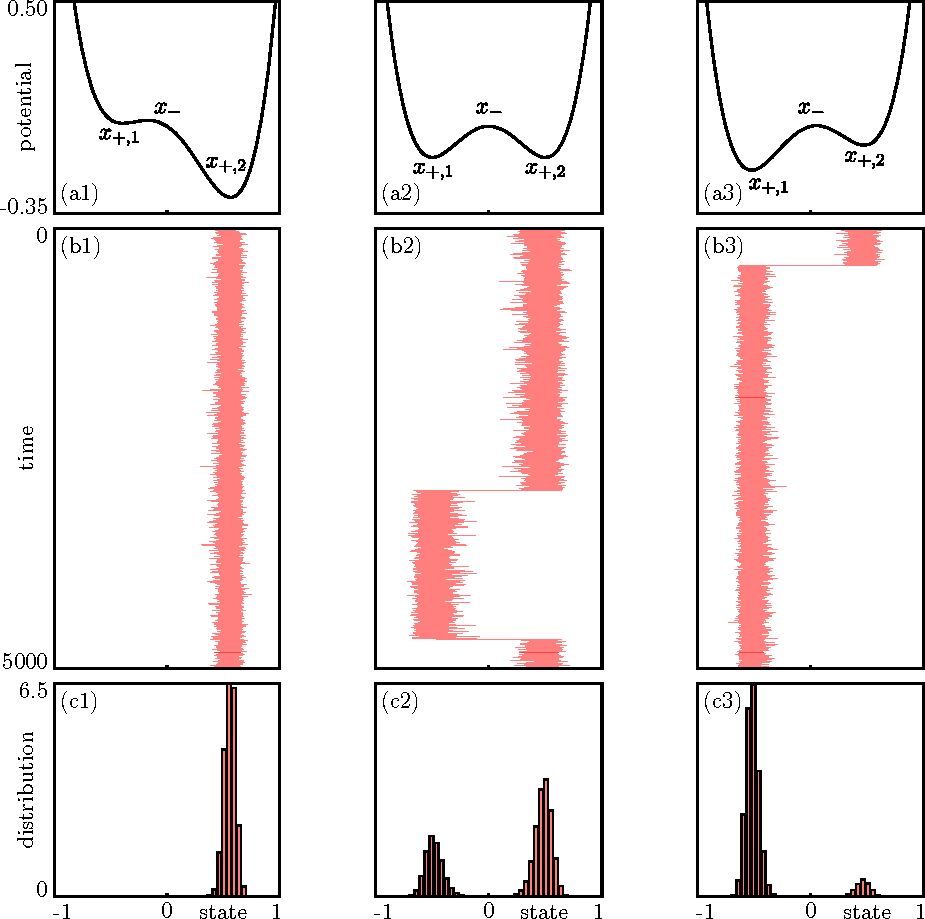
\includegraphics[keepaspectratio, width=\textwidth]{../figures/double_well_potential.pdf}
    \caption{Different configurations of a generic double-well potential leading to qualitatively different solutions of \eqref{eq:langevin} and bi--modal stationary distributions \eqref{eq:boltzmann_distribution}.
      Panels (a1-a3): shape of the confining potential with local minima $x_{+,1}$, $x_{+,2}$ and local maximum $x_-$.
      Panels (b1-b3): representative sample paths of \eqref{eq:langevin} for a particle starting from the rightmost local minimum $x_{+,2}$.
             Panels (c1-c3): empirical stationary distribution of the above timeseries depicted as histograms of homogeneous bin width.}
    \label{fig:double_well_potential}
\end{figure}
%
\subsection{The Ornstein--Uhlenbeck process}\label{subsec:oup}
One of the simplest SDEs that can be considered takes the form 
%
\begin{equation}\label{eq:oup}
  dX_{t} = \omega(\tilde{x} - X_{t})dt + \sqrt{2D}dW_{t},
\end{equation}
%
where the linear coefficient $\omega>0$ is somehow associated to the characteristic relaxation time of the process and $\tilde{x}\in\mathbb{R}$ is a shift in the coordinate of the state of the process $X_t$.
Notice that \eqref{eq:oup} can be written in Langevin form \eqref{eq:langevin} with the quadratic polynomial $V(x) = \omega(x - \tilde{x})^2/2$ as its potential. 
The solution of \eqref{eq:oup} is a so--called \emph{Ornstein--Uhlenbeck process} (OUP) and it can be found by variation of constants
%
\begin{equation}\label{eq:oup_solution}
  X_{t} = \tilde{x} + \exp(-\omega t)(x_0 - \tilde{x}) + \sqrt{2D}\int_{0}^{t}\exp\bigl(-\omega(t - s)\bigr)dW_s,
\end{equation}
%
where $X_0=x_0$ is the initial condition of the process.
The OUP is often called \emph{mean--reverting} in the sense that, in the long--run, such initial condition $x_0$ reverts back to the mean $\tilde{x}$.
This can be seen by considering the first two moments of \eqref{eq:oup_solution}
%
\begin{align*}
  \E[X_t] &= \tilde{x} + \exp(-\omega t)(x_0 - \tilde{x}), \\
  \text{Var}[X_t] &= \frac{D}{\omega}\bigl(1 - \exp(-2\omega t)\bigr) ,
\end{align*}
%
which, in the asymptotic limit $t\to\infty$, reduce to
%
\begin{equation}\label{eq:oup_variance}
  \E[X_t] \to \tilde{x}\quad \text{and} \quad \text{Var}[X_t] \to D/\omega.
\end{equation}
%
In the same long--run asymptote, the OUP admits a Boltzmann--like distribution of the form \eqref{eq:boltzmann_distribution} solving the stationary Fokker--Planck equation
%
\begin{equation}\label{eq:oup_distribution}
  p(x) = \sqrt{\frac{\omega}{2\pi D}}\exp\bigg(-\frac{\omega(\tilde{x} - x)^{2}}{2D}\bigg)\,,
\end{equation}
%
which is a Gaussian distribution with mean and variance given by \eqref{eq:oup_variance}.

The OUP plays a major role in the context of critical transitions and the prediction of CSD.  
The reason for this is that \eqref{eq:oup_solution} can be used to approximate the long--term behaviour of a variety of more complex, nonlinear processes (that is SDEs for which the drift term $f$ is nonlinear in $X_t$).
To see that, let us consider the case of a saddle--node normal form with additive noise
%
\begin{equation}\label{eq:saddle_node_normal_form}
  dX_{t} = (-\mu-X_{t}^{2})dt + \sqrt{2D}dW_{t},
\end{equation}
%
with the drift term $f(x;\mu) = -\mu - x^2$ being quadratic in $x$.
This nonlinear SDE is the centerpiece of a significant portion of the existing literature on critical transitions and early--warning signals and it will be used extensively throughout this thesis for the derivation of most of the results with little loss in generality (see \S~\ref{sec:dynamical_systems} for more details regarding this).
Notice that \eqref{eq:saddle_node_normal_form} can be rewritten in Langevin form \eqref{eq:langevin} with a cubic polynomial $V(x;\mu) = \mu x + x^3/3$ as its potential.

As discussed in \S~\ref{sec:framework}, for any strictly negative values of $\mu$, the quadratic drift term has two equilibria $x_{\pm}(\mu)=\pm\sqrt{-\mu}$, which also correspond to the local minimum and local maximum of $V$ respectively.
Let us assume that $X_t$ is a solution of the initial value problem \eqref{eq:ivp} for \eqref{eq:saddle_node_normal_form} starting at $X_0 = x_+(\mu_0)$ for some fixed $\mu_0\ll0$.
Provided a finite time horizon $T>0$ and a relatively small noise intensity $D\ll1$, the solution of such initial value problem can be written as $X_t = x_+ + Z_t$, which decomposes the stochastic process $X_t$ into a constant, deterministic component $x_+$ and a time--homogeneous, random component $Z_t$.
This decomposition allows us to describe the stochastic fluctuations of the solution around the stable equilibrium $x_+$ of the saddle--node normal form for a fixed but finite amount of time $T>0$.
Thus, by expanding $f$ around $x_+(\mu_0)$, we find
%
\begin{equation}\label{eq:taylor_expansion}
  f(X_t;\mu_0) = f\bigl(x_+(\mu_0);\mu_0\bigr) + Df\bigl(x_+(\mu_0);\mu_0\bigr)\bigl(X_t - x_+(\mu_0)\bigr) + o\bigr(|X_t - x_+(\mu_0)|\bigr),
\end{equation}
%
where the first term on the right--hand side vanishes by definition.
Substituting \eqref{eq:taylor_expansion} into \eqref{eq:saddle_node_normal_form}, and noting that $dX_t = dZ_t + dx_+ = dZ_t$, gives us
%
\begin{equation}\label{eq:oup_sn}
  dZ_t = JZ_tdt + \sqrt{2D}dW_t,
\end{equation}
%
where $J\coloneqq Df\bigl(x_+(\mu_0);\mu_0\bigr)$ quantifies the Jacobian of $f$ at $x=x_+(\mu_0)$.
It is evident that \eqref{eq:oup_sn} is an OUP of the form \eqref{eq:oup} with linear coefficient $\omega = -J = 2\sqrt{-\mu_0}$ and with no shift $\tilde{x} = 0$.
Written explicitly in the original coordinate system, it reads
%
\begin{equation}\label{eq:shifted_oup_sn}
  dX_t = 2\sqrt{-\mu_0}\bigl(\sqrt{-\mu_0} - X_t\bigr)dt + \sqrt{2D}dW_t,
\end{equation}
%
for which the asymptotic mean and variance given by \eqref{eq:oup_variance}
%
\begin{equation}\label{eq:sn_variance}
  \E[X_t]\to\sqrt{-\mu_0}\quad \text{and} \quad \text{Var}[X_t]\to D/2\sqrt{-\mu_0}.
\end{equation}
%
are attained by a sample--path in the long--run as shown by Monte Carlo simulations depicted in Figure~\ref{fig:oup_approximation}
%
\begin{figure}[!t]
    \centering 
    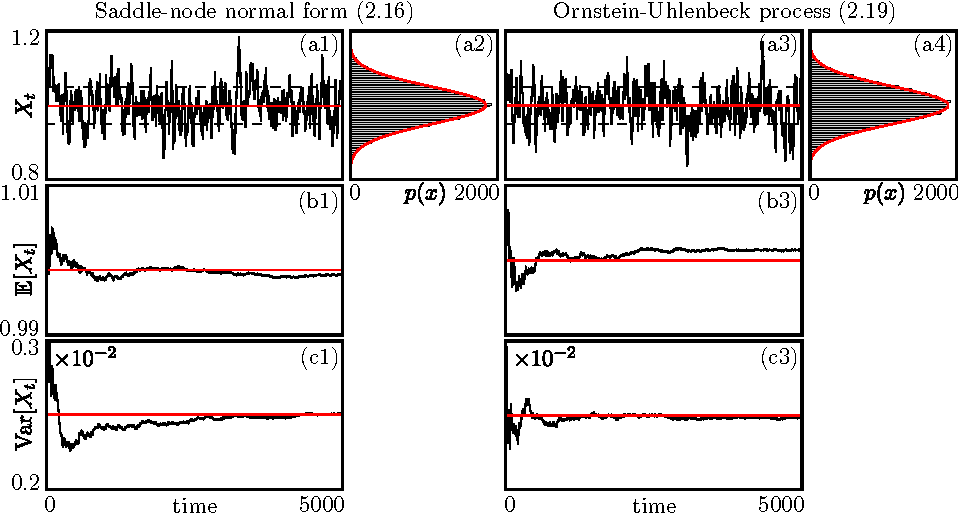
\includegraphics[keepaspectratio, width=\textwidth]{../figures/oup_approximation.pdf}
    \caption{Comparison of the long--run statistics of an OUP \eqref{eq:oup_solution} and a sample--path solving the time--homogeneous saddle--node normal form \eqref{eq:saddle_node_normal_form}.
      Panels (a1, a3): sample--paths (black curves) of the respective initial value problems with long--run mean (red line) and standard deviation (dashed black lines) provided in \eqref{eq:oup_variance}.
      Panels (a2, a4): empirical distribution (gray histograms) of the sample--paths with the stationary distribution (red curve) provided in \eqref{eq:boltzmann_distribution}.
      Panels (b1, b3): convergence of the sample mean (black curve) to the mean \eqref{eq:oup_variance} of the stationary distribution (red line) in the long--run.
      Panels (c1, c3): convergence of the sample variance (black curve) to the variance \eqref{eq:oup_variance} of the stationary distribution (red line) in the long--run.}
    \label{fig:oup_approximation}
\end{figure}

Notice that \eqref{eq:sn_variance} provides a mathematical underpinning of using the increase in variance as a precurson of CSD.
As the saddle--node bifurcation is approached $\mu_0\to0$, which implies that $\text{Var}[X_t]\to+\infty$, providing the blow--up that justifies the adoption of the timeseries variance as an early--warning signal.

\subsection{Large deviations theory}\label{subsec:ldt}
In statistical mechanics, Kramer's formula quantifies the rate at which particles escape across potential barriers when subject to Langevin's equation of motion \eqref{eq:langevin}.
Kramer's formula is sometimes expressed as the reciprocal of the escape time, usually referred to as the (mean) first exit time.
Different derivations of the formula are available in the literature; we thus redirect the readers to \cite{Berglund2013} for a concise overview.
It must be noted that, while limitations on Kramer's law vailidity exist (see \cite{Berglund2013}), our assumptions of stationary, $1-$dimensional dynamics subject to small, additive white noise fall within the applicability cases.
 
Given a double-well potential $V$ with desirable local minimum (stable equilibrium) $x=a$ and local maximum (unstable equilibrium) $x=b$, the rate at which particles, starting at $x=a$ and subject to white noise of intensity $\sqrt{2D}$, will escape over the saddle $x=b$ is given by
 
\begin{equation}\label{eq:kramer_escape_formula}
        R_{K} = \frac{\sqrt{|V''(x_-)|V''(x_+)}}{2\pi}\exp\bigg(-\frac{\Delta V}{D}\bigg)\,,
\end{equation}
%
where $\Delta V_{a\to b} = V(b) - V(a)$ quantifies the potential barrier that the Langevin overdamped particle has to overcome in order to escape, and $V''(a),V''(b)$ quantify the local curvature of $V$ around the well and the hilltop respectively.
%
The large deviation principle applied to the saddle--node normal form \eqref{eq:saddle_node_normal_form} gives
%
\begin{equation}\label{eq:ldp_saddle_node}
  R(\mu) = \exp\bigl(-\Delta V(\mu)\bigr) = \dots
\end{equation}

\section{Dynamical systems}\label{sec:dynamical_systems}
Introduce the autonomous saddle-node normal form and an example of coordinate transformations for the saddle-node bifurcation theorem.
Extend it to the dynamic case with the notion of pullback attractors.

\subsection{Geometric singular perturbation theory}\label{subsubsec:gspt}
Main results of Fenichel theory.
